% !TEX TS-program = pdflatex
% !TEX encoding = UTF-8 Unicode

% This is a simple template for a LaTeX document using the "article" class.
% See "book", "report", "letter" for other types of document.

\documentclass[11pt]{article} % use larger type; default would be 10pt

\usepackage[utf8]{inputenc} % set input encoding (not needed with XeLaTeX)

%%% Examples of Article customizations
% These packages are optional, depending whether you want the features they provide.
% See the LaTeX Companion or other references for full information.

%%% PAGE DIMENSIONS
\usepackage{geometry} % to change the page dimensions
\geometry{a4paper} % or letterpaper (US) or a5paper or....
% \geometry{margin=2in} % for example, change the margins to 2 inches all round
% \geometry{landscape} % set up the page for landscape
%   read geometry.pdf for detailed page layout information

\usepackage{graphicx} % support the \includegraphics command and options

% \usepackage[parfill]{parskip} % Activate to begin paragraphs with an empty line rather than an indent

%%% PACKAGES
\usepackage{tikz}
\usepackage{dsfont}
\usepackage{pgfplots}
\usepackage{booktabs} % for much better looking tables
\usepackage{array} % for better arrays (eg matrices) in maths
\usepackage{paralist} % very flexible & customisable lists (eg. enumerate/itemize, etc.)
\usepackage{verbatim} % adds environment for commenting out blocks of text & for better verbatim
\usepackage{subfig} % make it possible to include more than one captioned figure/table in a single float
% These packages are all incorporated in the memoir class to one degree or another...

%%% HEADERS & FOOTERS
\usepackage{fancyhdr} % This should be set AFTER setting up the page geometry
\pagestyle{fancy} % options: empty , plain , fancy
\renewcommand{\headrulewidth}{0pt} % customise the layout...
\lhead{}\chead{}\rhead{}
\lfoot{}\cfoot{\thepage}\rfoot{}

%%% SECTION TITLE APPEARANCE
\usepackage{sectsty}
\allsectionsfont{\sffamily\mdseries\upshape} % (See the fntguide.pdf for font help)
% (This matches ConTeXt defaults)

%%% ToC (table of contents) APPEARANCE
\usepackage[nottoc,notlof,notlot]{tocbibind} % Put the bibliography in the ToC
\usepackage[titles,subfigure]{tocloft} % Alter the style of the Table of Contents
\renewcommand{\cftsecfont}{\rmfamily\mdseries\upshape}
\renewcommand{\cftsecpagefont}{\rmfamily\mdseries\upshape} % No bold!

%%% END Article customizations

%%% The "real" document content comes below...

\title{Mahavier}
\author{Ethan Schaffer}
\date{Due 10/13/2016} % Activate to display a given date or no date (if empty),
         % otherwise the current date is printed 
\newcommand\tab[1][1cm]{\hspace*{#1}}
\newcommand\ang{$\theta$}
\newcommand\unitcircle{
\draw[step=1cm,gray,very thin] (-3,-3) grid (3,3); %grid body
\draw[thick, dashed] (-4,0) -- (0,0); %grid line
\draw[thick, dashed] (0,-4) -- (0,0); %grid line
\draw[thick, dashed] (0,0) -- (4,0) node[anchor=north west] {x}; %axis
\draw[thick, dashed] (0,0) -- (0,4) node[anchor=south east] {y}; %axis
\draw [thick] (0,0) circle (2cm);
\draw [dashed] (-1.4,-1.4) -- (1.4, 1.4);
\draw [dashed] (-1.4,1.4)--(1.4,-1.4);
\draw [dashed] (-1, -1.73) -- (1, 1.73);
\draw [dashed] (1, -1.73) -- (-1, 1.73);
\draw [dashed] (-1.73, -1) -- (1.73, 1);
\draw [dashed] (1.73, -1) -- (-1.73, 1);
\draw (1.5, 2.5) node [rotate=60] {($\frac{1}{2}, \frac{\sqrt{3}}{2}$)};
\draw (2.5, 1.5) node [rotate=30] {($\frac{\sqrt{3}}{2}, \frac{\sqrt{1}}{2}$)};
\draw (-1.75, -2.75) node [rotate=60] {($-\frac{1}{2}, -\frac{\sqrt{3}}{2}$)};
\draw (-2.75, -1.5) node [rotate=30] {($-\frac{\sqrt{3}}{2}, -\frac{\sqrt{1}}{2}$)};
\draw (1.5, -2.5) node [rotate=-60] {($\frac{\sqrt{3}}{2}, -\frac{1}{2}$)};
\draw (2.5, -1.5) node [rotate=-30] {($\frac{1}{2}, -\frac{\sqrt{3}}{2}$)};
\draw (-1.5, 2.5) node [rotate=-60] {($-\frac{\sqrt{3}}{2}, \frac{1}{2}$)};
\draw (-2.5, 1.5) node [rotate=-30] {($-\frac{1}{2}, \frac{\sqrt{3}}{2}$)};
\draw (2.25, 2.25) node[rotate=45] {($\frac{\sqrt{2}}{2}$, $\frac{\sqrt{2}}{2}$)};
\draw (-2.25,2.25) node[rotate=-45] {($-\frac{\sqrt{2}}{2}$, $\frac{\sqrt{2}}{2}$)};
\draw (2.25,-2.25) node[rotate=-45] {($\frac{\sqrt{2}}{2}$, $-\frac{\sqrt{2}}{2}$)};
\draw (-2.25,-2.25) node[rotate=45] {($-\frac{\sqrt{2}}{2}$, $-\frac{\sqrt{2}}{2}$)};
\draw(-.25, -2.5) node[rotate=90] {(0,-1)};
\draw(2.5, -.25) node {(1,0)};
\draw(.25, 2.5) node[rotate=90] {(0,1)};
\draw(-2.5, 0.25) node {(-1,0)};
}
\newcommand\unitcirclenolines{
\draw[step=1cm,gray,very thin] (-2,-2) grid (2,2); %grid body
\draw[thick, dashed] (-2,0) -- (0,0); %grid line
\draw[thick, dashed] (0,-2) -- (0,0); %grid line
\draw[thick, dashed] (0,0) -- (2,0) node[anchor=north west] {x}; %axis
\draw[thick, dashed] (0,0) -- (0,2) node[anchor=south east] {y}; %axis
\draw [thick] (0,0) circle (1cm);
}

\begin{document}
\maketitle

\begin{comment}

\end{comment}

\large{All units circle graphs are labelled in the counter-clockwise direction}

\textbf{Definition 1. The unit circle is the circle centered at the origin and of radius one}
\section{Problem 1}
\textit{Graph the unit circle, and subdivide it into eight arcs of equal length such that
one division lies at the point (1,0). Working in a counter-clockwise direction, determine
the distance along the unit circle from the point (1,0) to each of the divisions, and label
each division with this distance}\\
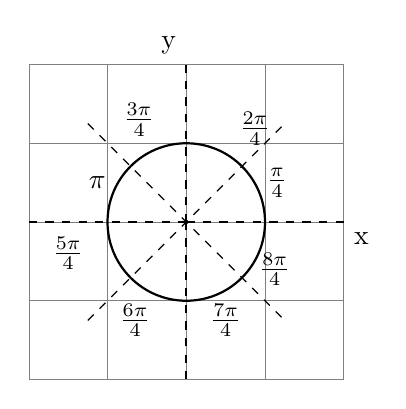
\begin{tikzpicture}
\draw[step=1cm,gray,very thin] (-2,-2) grid (2,2); %grid body
\draw[thick, dashed] (-2,0) -- (0,0); %grid line
\draw[thick, dashed] (0,-2) -- (0,0); %grid line
\draw[thick, dashed] (0,0) -- (2,0) node[anchor=north west] {x}; %axis
\draw[thick, dashed] (0,0) -- (0,2) node[anchor=south east] {y}; %axis

\draw [thick] (0,0) circle (1cm);
\draw [dashed] (-1.25, -1.25) -- (1.25, 1.25); \draw [dashed] (-1.25, 1.25) -- (1.25, -1.25);

\draw (.9,.5) node[anchor= west]{$\frac{\pi}{4}$}; \draw (.55,.85) node[anchor=south west]{$\frac{2\pi}{4}$};
\draw(-.6, 1.3)  node {$\frac{3\pi}{4}$}; 				   \draw(-.9,.5) node [anchor=east] {$\pi$};
\draw (-1.5,-.4) node{$\frac{5\pi}{4}$};				   \draw(-.65,-1.25) node {$\frac{6\pi}{4}$};
\draw (.5,-1.25) node{$\frac{7\pi}{4}$};			   \draw (0.8,-.6)  node [anchor=west] {$\frac{8\pi}{4}$};
\end{tikzpicture}

\section{Problem 2}
\textit{Repeat the previous exercise using a total of twelve divisions.}
\\

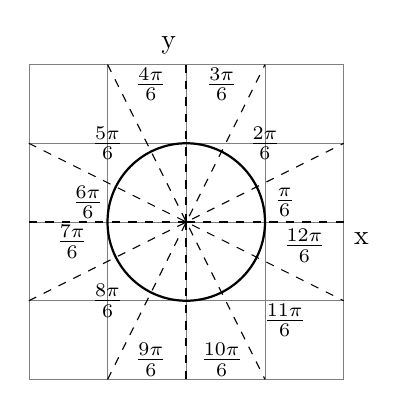
\begin{tikzpicture}
\draw[step=1cm,gray,very thin] (-2,-2) grid (2,2); %grid body
\draw[thick, dashed] (-2,0) -- (0,0); \draw[thick, dashed] (0,-2) -- (0,0); %grid lines
\draw[thick, dashed] (0,0) -- (2,0) node[anchor=north west] {x}; %axis
\draw[thick, dashed] (0,0) -- (0,2) node[anchor=south east] {y}; %axis

\draw [thick] (0,0) circle (1cm);
\draw [dashed] (-1, -2) -- (1, 2); \draw [dashed] (-2, -1) -- (2, 1);
\draw [dashed] (-1, 2) -- (1, -2); \draw [dashed] (-2, 1) -- (2, -1);

\draw (1.25,.25) node {$\frac{\pi}{6}$};			 \draw (1,1) node {$\frac{2\pi}{6}$};
\draw (.45,1.75) node {$\frac{3\pi}{6}$};			 \draw (-.45,1.75) node {$\frac{4\pi}{6}$};
\draw (-1,1) node {$\frac{5\pi}{6}$}; 	 			 \draw (-1.25,.25) node {$\frac{6\pi}{6}$};
\draw (-1.45,-.25) node {$\frac{7\pi}{6}$};	 \draw (-1,-1) node {$\frac{8\pi}{6}$};
\draw (-.45,-1.75) node {$\frac{9\pi}{6}$};	 \draw (.45,-1.75) node {$\frac{10\pi}{6}$};
\draw (1.25,-1.25) node {$\frac{11\pi}{6}$};	 \draw (1.5,-.3) node {$\frac{12\pi}{6}$};
\end{tikzpicture}


\section{Problem 3}
\textit{Repeat the previous two exercises, using a circle centered at the origin and of
radius two.}
\subsection{Subsection 1}

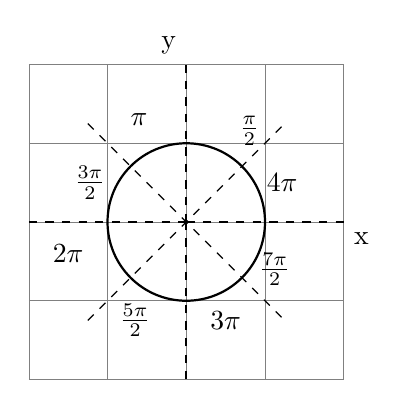
\begin{tikzpicture}
\draw[step=1cm,gray,very thin] (-2,-2) grid (2,2); %grid body
\draw[thick, dashed] (-2,0) -- (0,0); %grid line
\draw[thick, dashed] (0,-2) -- (0,0); %grid line
\draw[thick, dashed] (0,0) -- (2,0) node[anchor=north west] {x}; %axis
\draw[thick, dashed] (0,0) -- (0,2) node[anchor=south east] {y}; %axis

\draw [thick] (0,0) circle (1cm);
\draw [dashed] (-1.25, -1.25) -- (1.25, 1.25); \draw [dashed] (-1.25, 1.25) -- (1.25, -1.25);

\draw (.9,.5) node[anchor= west]{4$\pi$};	\draw (.55,.85) node[anchor=south west]{$\frac{\pi}{2}$};
\draw(-.6, 1.3)  node {$\pi$}; 				   		\draw(-.9,.5) node [anchor=east] {$\frac{3\pi}{2}$};
\draw (-1.5,-.4) node{2$\pi$};					   	\draw(-.65,-1.25) node {$\frac{5\pi}{2}$};
\draw (.5,-1.25) node{3$\pi$};				   		\draw (0.8,-.6)  node [anchor=west] {$\frac{7\pi}{2}$};
\end{tikzpicture}

\subsection{Subsection 2}
\textit{Draw a units circle with twelve unique arcs and a radius of length 2 units.} \\

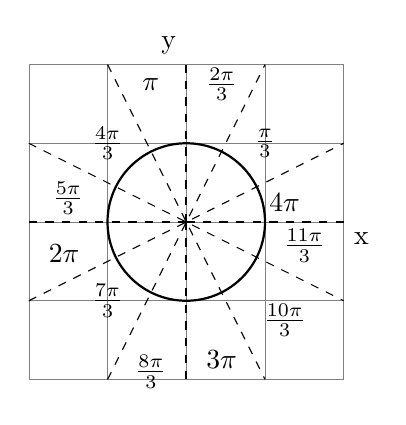
\begin{tikzpicture}
\draw[step=1cm,gray,very thin] (-2,-2) grid (2,2); %grid body
\draw[thick, dashed] (-2,0) -- (0,0); \draw[thick, dashed] (0,-2) -- (0,0); %grid lines
\draw[thick, dashed] (0,0) -- (2,0) node[anchor=north west] {x}; %axis
\draw[thick, dashed] (0,0) -- (0,2) node[anchor=south east] {y}; %axis

\draw [thick] (0,0) circle (1cm);
\draw [dashed] (-1, -2) -- (1, 2); \draw [dashed] (-2, -1) -- (2, 1);
\draw [dashed] (-1, 2) -- (1, -2); \draw [dashed] (-2, 1) -- (2, -1);

\draw (1.25,.25) node {$4\pi$};			 				\draw (1,1) node {$\frac{\pi}{3}$};
\draw (.45,1.75) node {$\frac{2\pi}{3}$};			 \draw (-.45,1.75) node {$\pi$};
\draw (-1, 1) node {$\frac{4\pi}{3}$}; 	 			 \draw (-1.5,.3) node {$\frac{5\pi}{3}$};
\draw (-1.55,-.4) node {$2\pi$};	 					 \draw (-1,-1) node {$\frac{7\pi}{3}$};
\draw (-.45,-1.9) node {$\frac{8\pi}{3}$};			 \draw (.45,-1.75) node {$3\pi$};
\draw (1.25,-1.25) node {$\frac{10\pi}{3}$};	 \draw (1.5,-.3) node {$\frac{11\pi}{3}$};
\end{tikzpicture}
\\
\tab \textbf{Definition 2.} An angle is a subset of the plane consisting of two distinct rays (or two
distinct line segments) with a common endpoint called the vertex.\\
\tab \textbf{Definition 3.} An angle in standard position is an angle where one of the two rays is the
positive x-axis. This ray is referred to as the initial side of the angle. The other ray is
referred to as the terminal side of the angle.\\
\tab \textbf{Definition 4}. Given a circle centered at the origin and an angle in standard position,
let P1 be the intersection of the circle with the initial side of the angle, and let P2 be the
intersection of the circle with the terminal side of the angle. 
The arc associated with the angle is the portion of the circle traced by a point traversing the circle in a counterclockwise
direction from the point P1 to the point P2.\\
\tab \textbf{Definition 5.} Given a circle centered at the origin and an angle in standard position, the
radian measure of the angle is the ratio of the length of the arc associated with the angle
to the radius of the circle.\\

\section{Problem 4}
\textit{Determine the radian measure of each angle illustrated below.} \\
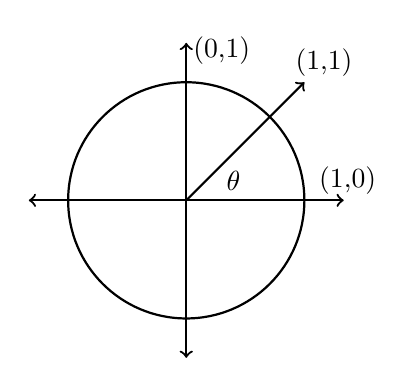
\begin{tikzpicture}
\draw[thick, <->] (0,-2) -- (0,2); \draw[thick, <->] (-2,0) -- (2,0); %axes
\draw [thick] (0,0) circle (1.5cm);
\draw (2.05, .25) node {(1,0)}; \draw (.45, 1.9) node {(0,1)};
\draw[thick, ->] (0,0) -- (1.5,1.5); \draw(.6, .25) node {$\theta$};
\draw (1.75, 1.75) node{(1,1)};
\end{tikzpicture}
\\
%Text Here
For the above figure, we know that the radian measure is equal to $\frac{Arc Length}{radius}$. 
We can look up the arc length in our solution to problem 3.2.
In this case, that is $\frac{\pi}{4}$/1, which is simply \textbf{$\frac{\pi}{4}$}.
\\
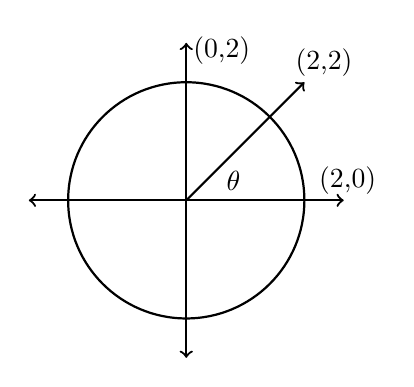
\begin{tikzpicture}
\draw[thick, <->] (0,-2) -- (0,2); \draw[thick, <->] (-2,0) -- (2,0); %axes
\draw [thick] (0,0) circle (1.5cm);
\draw (2.05, .25) node {(2,0)}; \draw (.45, 1.9) node {(0,2)};
\draw[thick, ->] (0,0) -- (1.5,1.5); \draw(.6, .25) node {$\theta$};
\draw (1.75, 1.75) node{(2,2)};
\end{tikzpicture}
\\
%Text Here
For the above figure, we know that the radian measure is equal to $\frac{Arc Length}{radius}$. 
We can look up the arc length in our solution to problem 3.2.
In this case, that is $\frac{\pi}{2}$/2, which \textit{also} equal to \textbf{$\frac{\pi}{4}$}.
Based on this, we can actually conclude that the radius of a circle does not affect the radian measurement of any angle. 
This is just like how the radius of a circle does not affect it's degree measure.

\section{Problem 5}
\textit{Given an angle, not necessarily in standard position, make up a definition for
the radian measure of the angle.}
\\
We know that the angle that is an entire circle, in radians, is equal to 2$\pi$. In degrees, that angle is 360 degrees. 
Based on this, we can determine a proportion for the ratios of these two angles. That relationship would be 360 = 2$\pi$. 
So, whatever portion of 360 any angle \textit{a} would take up, it would take up that same portion of 2$\pi$. 
This means we can use the equation \\ 
\begin{displaymath} degrees_\theta = \frac{360*radians_\theta}{2\pi} \end{displaymath} 
\\ to express the relationship between the degree and radian measure of any angle.\\
\\
\tab \textbf{Definition 6.} Given a circle centered at the origin and an angle in standard position, the
degree measure of the angle is $\frac{360}{2\pi}$ times the radian measure of the angle.
Historically, the circle was evenly divided into 360 arcs, and an angle was said to have
degree measure $\theta$ if the terminal side of the angle intersected the circle at the $\theta$th division.
I have read two explanations of this – the choice of 360 was because it was believed there
were 360 days in a year, or because much mathematics was done based on multiples of 60.
If pressed, I could probably come up with a source supporting these statements.
\\
\tab \textbf{Definition 7.} A right triangle is a triangle that has one angle with degree measure 90.
\\
\tab \textbf{Theorem 1.} The sum of the degree measures of the interior angles of a triangle is 180.
\\
\tab \textbf{Definition 8.} The hypotenuse of a right triangle is the side that is not adjacent to the angle
of degree measure 90.
\\
\tab \textbf{Theorem 2: Pythagorean Theorem:} Given a right triangle with sides of length a, b, and
c, where c is the length of the hypotenuse, we have $a^2 +b^2 = c^2$.
Notation: If the degree measure of an angle is $\theta$, then we will say that such an angle has
measure $\theta$ degrees.

\section{Problem 6}
\textit{Determine the degree measure of each angle in the previous illustration}
\\
\tab We have already shown that both angles in the previous illustration have a measure of $\frac{\pi}{4}$. So, we know that these angles must be equal to one another, and must work for our formula $degrees_\theta = \frac{360*radians_\theta}{2\pi}$. This equation tells us that \textbf{$degrees_\theta$ = 45$^{\circ}$}. Based on what I already know about triangles, this makes sense. 

\section{Problem 7}
\textit{Graph the unit circle, and the angle in standard position whose measure is 150 degrees.}
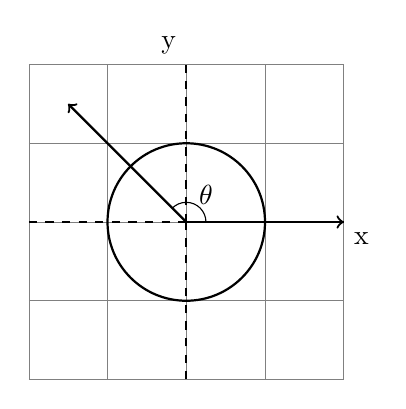
\begin{tikzpicture}
\draw[step=1cm,gray,very thin] (-2,-2) grid (2,2); %grid body
\draw[thick, dashed] (-2,0) -- (0,0); \draw[thick, dashed] (0,-2) -- (0,0); %grid lines
\draw[thick, dashed] (0,0) -- (2,0) node[anchor=north west] {x}; %axis
\draw[thick, dashed] (0,0) -- (0,2) node[anchor=south east] {y}; %axis
\draw [thick] (0,0) circle (1cm);
\draw [thick, ->] (0,0) -- (2,0);
\draw [thick, ->] (0,0) -- (-1.5,1.5);
\draw (.25, 0) arc (0:135:.25);
\draw (.25, .35) node {$\theta$};
\end{tikzpicture}

\section{Problem 8}
\textit{. Graph the unit circle, and the angle in standard position that has measure $\frac{\pi}{4}$ radians.}
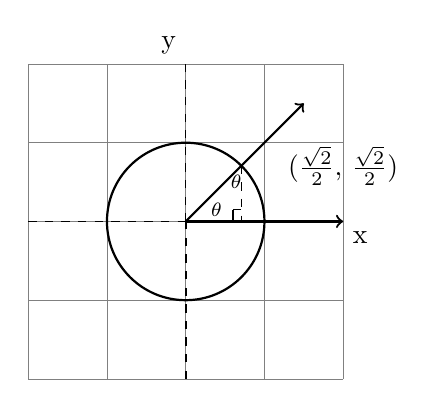
\begin{tikzpicture}
\draw[step=1cm,gray,very thin] (-2,-2) grid (2,2); %grid body
\draw[thin, dashed] (-2,0) -- (0,0); \draw[thick, dashed] (0,-2) -- (0,0); %grid lines
\draw[thin, dashed] (0,0) -- (2,0) node[anchor=north west] {x}; %axis
\draw[thin, dashed] (0,0) -- (0,2) node[anchor=south east] {y}; %axis
\draw [thick] (0,0) circle (1cm);
\draw [thick, ->] (0,0) -- (2,0);
\draw [thick, ->] (0,0) -- (1.5,1.5);
\draw (2, .707) node  {($\frac{\sqrt{2}}{2}$, $\frac{\sqrt{2}}{2}$)};
\draw [dashed] (.707, .707) -- (.707, 0);
%Right angle
\draw [thin] (.6, 0) -- (.6, .15);
\draw [thin] (.6, .15) -- (.707, .15);
%Symbols
\draw (.4, .15) node {$ _\theta$};
\draw (.65, .5) node {$ _\theta$};

\end{tikzpicture}
\\
\textit{What are the xy-coordinates of the point that is the intersection of the terminal side of this angle with the unit circle?}\\
\tab The xy-coordinates in question have been labelled above. We know that the hypotenuse must be of length 1, because it is the radius of our units circle. We also know that each angle must be equal to one another. So, each leg must also be equal to the other. This means that when we apply the \textbf{Pythaorean Theorem}, we find that each leg of the triangle must be of length $\sqrt{\frac{1}{2}}$.  In another form (that we will use from now on), we see that $\sqrt{\frac{1}{2}}$ = $\frac{\sqrt{2}}{2}$.

\section{Problem 9}
\textit{Graph the unit circle, and the angle in standard position that has measure $\frac{\pi}{3}$ radians.} \\
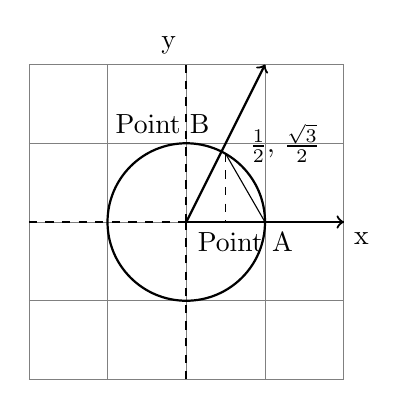
\begin{tikzpicture}
\draw[step=1cm,gray,very thin] (-2,-2) grid (2,2); %grid body
\draw[thick, dashed] (-2,0) -- (0,0); \draw[thick, dashed] (0,-2) -- (0,0); %grid lines
\draw[thick, dashed] (0,0) -- (2,0) node[anchor=north west] {x}; %axis
\draw[thick, dashed] (0,0) -- (0,2) node[anchor=south east] {y}; %axis
\draw [thick] (0,0) circle (1cm);
\draw [thick, ->] (0,0) -- (2,0);
\draw [thick, ->] (0,0) -- (1,2);
\draw [dashed] (.5, .866) -- (.5, 0);
\draw (.5, .866) -- (1, 0);
\draw(-.3, 1.25) node {Point B};
\draw (.75, -.25) node {Point A};

\draw (1.25, 1) node {$1\over 2$, $\sqrt{3} \over 2$};
\end{tikzpicture}
\\
\textit{What are the xy-coordinates of the point that is the intersection of the terminal side of this angle with the unit circle?} \\
\tab We can draw the dotted line from the point in question down to the x axis, and it creates a triangle with a $60^{\circ}$  angle in the bottom left corner. 
We can mirror this triangle, then creating an equilateral triangle. 
We know that line AB bisects the triangle, so that Point A must be at (.5,0). 
Then, we can use the Pythagorean Theorem to find the height of the triangle. 
That value, $\frac{\sqrt{3}}{2}$, is the y-coordinate of Point B.
\textit{What is the length of the arc associated with this angle?} \\
\tab The length of the arc associated with this angle is $\frac{\pi}{3}$. We know this beause for any circle of radius one, the length of an arc is the same as the radian measure of it's cooresponding angle. 
This is actually the $definition_?$ of radian measure.

\section{Problem 10}
\textit{Graph a circle of radius 2 centered at the origin, and the angle in standard position so that the length of the arc associated with the angle is $\frac{3\pi}{2}$}
\\
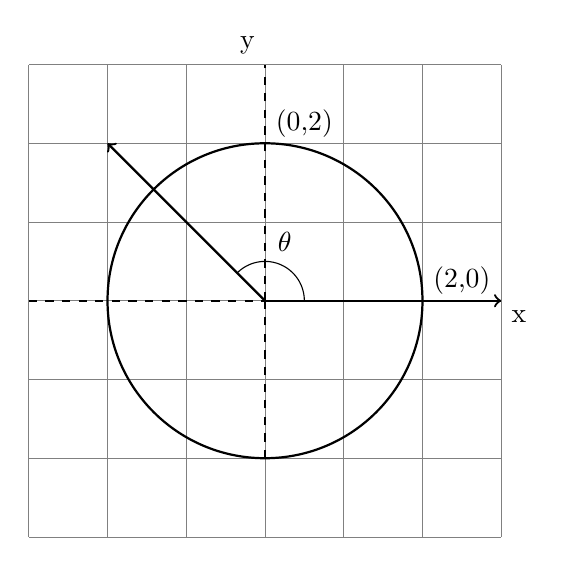
\begin{tikzpicture}
\draw[step=1cm,gray,very thin] (-3,-3) grid (3,3); %grid body
\draw[thick, dashed] (-3,0) -- (0,0); \draw[thick, dashed] (0,-2) -- (0,0); %grid lines
\draw[thick, dashed] (0,0) -- (3,0) node[anchor=north west] {x}; %axis
\draw[thick, dashed] (0,0) -- (0,3) node[anchor=south east] {y}; %axis
\draw [thick] (0,0) circle (2cm);
\draw [thick, ->] (0,0) -- (3,0);
\draw [thick, ->] (0,0) -- (-2,2);
\draw (.5,0) arc (0:135:.5);
\draw (.25, .75) node {$\theta$};
\draw (2.5, .25) node {(2,0)};
\draw (.5, 2.25) node {(0,2)};
\end{tikzpicture}
\\
\textit{What is the radian measure of this angle?}\\
\tab The radian measure of this angle is $\frac{\frac{3\pi}{2}}{2}$, which simplifies to $\frac{3\pi}{4}$. \\
\textit{What is the degree measure of this angle?}\\
\tab The degree measure of this angle, when calculated by our formula, is $135^{\circ}$.

\section{Problem 11}
\textit{Given a circle centered at the origin with radius 5 centimeters, and an angle in standard position with radian measure $\frac{7\pi}{4}$, determine the length of the arc associated with this angle.} 
\\ \tab The length of the arc would be 5 times the length of the arc on the unit circle, because the radius is 5 times as large. So, the arc's length would be $\frac{35\pi}{4}$. 

\section{Problem 12}
\textit{Suppose that a unicycle with a wheel of radius 9 inches is rolled 4 feet. Through what radian measure has one spoke on this wheel traveled? }\\
\tab The spoke of the wheel would travel a total of $\frac{48}{18\pi}$ radians. 
\\ \textit{How many revolutions has the wheel made?} \\
\tab The wheel would make 5$\frac{1}{3}$ revolutions. 

\section{Problem 13}
\textit{Suppose that it took 2 seconds to roll the unicycle (described in the previous problem) 2 feet. What is the speed of the unicycle as measured in inches per second?}\\
\tab The speed of the unicycle is 12 inches per second. 
\\ \textit{As measured in radians per second?}\\
\tab The speed of the unicycle is 1$\frac{1}{3}$ radians per second.
\\ \textit{As measured in revolutions per second?}
\\
\tab The speed of the unicycle is $\frac{2}{3}$ of a revolution per second.

\section{Problem 14}
Given an angle of degree measure 270, determine the radian measure of the angle.
\tab The formula we already found can be applied here. 
\begin{displaymath} degrees_\theta = \frac{360*radians_\theta}{2\pi} \end{displaymath} 
\begin{displaymath} 270 = \frac{360*radians_\theta}{2\pi} \end{displaymath} 
\begin{displaymath} radians_\theta = \frac{3\pi}{2} \end{displaymath} 

\section{Problem 15} 
Given an angle of radian measure $\frac{2\pi}{3}$, determine the degree measure of this angle.
\tab The formula we already found can be applied here. 
\begin{displaymath} degrees_\theta = \frac{360*radians_\theta}{2\pi} \end{displaymath} 
\begin{displaymath} degrees_\theta = \frac{360*\frac{2\pi}{3}}{2\pi} \end{displaymath} 
\begin{displaymath} degrees_\theta = 120  \end{displaymath} 

The development above hinges on the choice of the counter-clockwise direction in the definition of the arc associated with the angle. 
\\ \tab An analogous series of definitions can be made using the clockwise direction.
From this point forward, we will use the convention that an angle measured in the clockwise direction from the positive x-axis will have negative measure and be referred to as a negative angle, while an angle measured in the counterclockwise direction from the positive x-axis will have a positive measure and be referred to as a positive angle.

\section{Problem 16}
Locate the point on the unit circle so that the angle formed by the radius of the circle containing this point and the positive x-axis is $\frac{-3\pi}{4}$ radians. What is the measure of this angle in degrees? \\
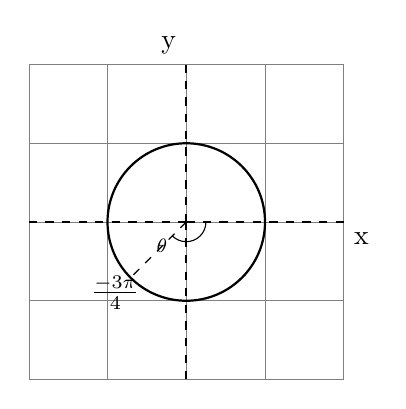
\begin{tikzpicture}
\draw[step=1cm,gray,very thin] (-2,-2) grid (2,2); %grid body
\draw[thick, dashed] (-2,0) -- (0,0); %grid line
\draw[thick, dashed] (0,-2) -- (0,0); %grid line
\draw[thick, dashed] (0,0) -- (2,0) node[anchor=north west] {x}; %axis
\draw[thick, dashed] (0,0) -- (0,2) node[anchor=south east] {y}; %axis

\draw [thick] (0,0) circle (1cm);
\draw [dashed] (0,0) -- (-.707, -.707);

\draw (-.9,-.9) node {$\frac{-3\pi}{4}$};
\draw (.25,0) arc(0:-135:.25);
\draw (-.3, -.3) node {$_\theta$};
\end{tikzpicture}
\\The measure of this angle in degrees is -135 degrees. This can be found through application of the formula we found earlier.

\section{Problem 17}
\textit{Given an angle of degree measure} -405, \textit{determine the radian measure of this angle.} \\
\tab The radian measure of the above angle, based on the formula, is $\frac{9\pi}{4}$ radians.

\section{Thank God We Get to Skip Problem 18}
I write enough essays for Mr. Snyder! 

\section{Problem 19} 
Determine the coordinates in the xy-plane of each point on the unit circle whose distance from the point (1,0) along the circle in a counter-clockwise direction is an integer multiple of $\frac{\pi}{4}$.\\
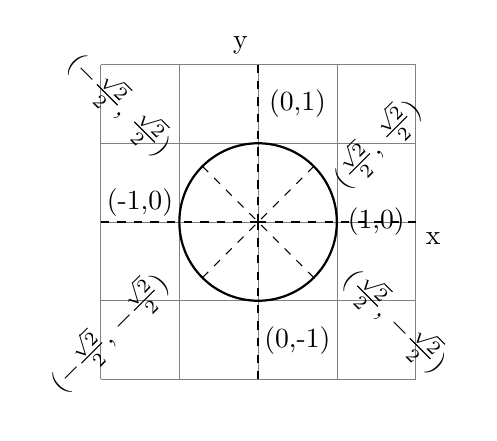
\begin{tikzpicture}
\draw[step=1cm,gray,very thin] (-2,-2) grid (2,2); %grid body
\draw[thick, dashed] (-2,0) -- (0,0); %grid line
\draw[thick, dashed] (0,-2) -- (0,0); %grid line
\draw[thick, dashed] (0,0) -- (2,0) node[anchor=north west] {x}; %axis
\draw[thick, dashed] (0,0) -- (0,2) node[anchor=south east] {y}; %axis

\draw [thick] (0,0) circle (1cm);
\draw [dashed] (-.707,-.707) -- (.707, .707);
\draw [dashed] (-.707,.707)--(.707,-.707);

\draw (1.5,1) node[rotate=45] {($\frac{\sqrt{2}}{2}$, $\frac{\sqrt{2}}{2}$)};
\draw (-1.75,1.5) node[rotate=-45] {($-\frac{\sqrt{2}}{2}$, $\frac{\sqrt{2}}{2}$)};
\draw (1.75,-1.25) node[rotate=-45] {($\frac{\sqrt{2}}{2}$, $-\frac{\sqrt{2}}{2}$)};
\draw (-1.9,-1.4) node[rotate=45] {($-\frac{\sqrt{2}}{2}$, $-\frac{\sqrt{2}}{2}$)};

\draw(.5, -1.5) node {(0,-1)};
\draw(1.5, 0) node {(1,0)};
\draw(.5, 1.5) node {(0,1)};
\draw(-1.5, 0.25) node {(-1,0)};

\end{tikzpicture}

\section{Problem 20}
Determine the coordinates in the xy-plane of each point on the unit circle such that the angle that is in standard position with terminal side containing the point has radian measure of an integer multiple of $\frac{\pi}{6}$.\\
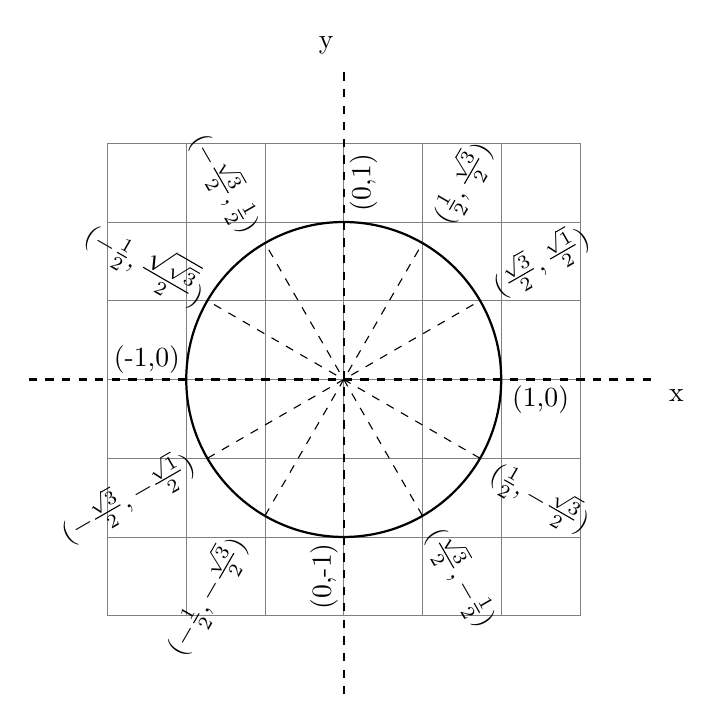
\begin{tikzpicture}
\draw[step=1cm,gray,very thin] (-3,-3) grid (3,3); %grid body
\draw[thick, dashed] (-4,0) -- (0,0); %grid line
\draw[thick, dashed] (0,-4) -- (0,0); %grid line
\draw[thick, dashed] (0,0) -- (4,0) node[anchor=north west] {x}; %axis
\draw[thick, dashed] (0,0) -- (0,4) node[anchor=south east] {y}; %axis
\draw [thick] (0,0) circle (2cm);
\draw [dashed] (-1, -1.73) -- (1, 1.73);
\draw [dashed] (1, -1.73) -- (-1, 1.73);
\draw [dashed] (-1.73, -1) -- (1.73, 1);
\draw [dashed] (1.73, -1) -- (-1.73, 1);
\draw (1.5, 2.5) node [rotate=60] {($\frac{1}{2}, \frac{\sqrt{3}}{2}$)};
\draw (2.5, 1.5) node [rotate=30] {($\frac{\sqrt{3}}{2}, \frac{\sqrt{1}}{2}$)};
\draw (-1.75, -2.75) node [rotate=60] {($-\frac{1}{2}, -\frac{\sqrt{3}}{2}$)};
\draw (-2.75, -1.5) node [rotate=30] {($-\frac{\sqrt{3}}{2}, -\frac{\sqrt{1}}{2}$)};
\draw (1.5, -2.5) node [rotate=-60] {($\frac{\sqrt{3}}{2}, -\frac{1}{2}$)};
\draw (2.5, -1.5) node [rotate=-30] {($\frac{1}{2}, -\frac{\sqrt{3}}{2}$)};
\draw (-1.5, 2.5) node [rotate=-60] {($-\frac{\sqrt{3}}{2}, \frac{1}{2}$)};
\draw (-2.5, 1.5) node [rotate=-30] {($-\frac{1}{2}, \frac{\sqrt{\sqrt{3}}}{2}$)};
\draw(-.25, -2.5) node[rotate=90] {(0,-1)};
\draw(2.5, -.25) node {(1,0)};
\draw(.25, 2.5) node[rotate=90] {(0,1)};
\draw(-2.5, 0.25) node {(-1,0)};
\end{tikzpicture}
\\
\\
\tab \textbf{Definition 9}\\
\textit{A function is a collection of points in the plane with the property that no two of these points lie in the same vertical line.}

You have probably seen the concept of a function denoted by such algebraic expressions as perhaps f(x)=$x^2$ or y=$x^2$.

These are not functions; rather, they are expressions that represent a function. 

The function itself is the collection of points (or ordered pairs) that you might graph to form a graphical representation of the function. 

Thus, I would say that we define a function f by the equation f(x)=$x^2$, and it is understood that f is the function consisting of the ordered pairs generated by the equation. 

Thus f ={(1,1),(2,4),(-3,9),\dots}. 

\textbf{Definition 10}
\\ \tab The first coordinates (x-coordinates) of all ordered pairs of a function f are referred to as the domain of f, while the second coordinates (y-coordinates) are referred to as the range of f.
In the next definitions, we will use the same type of notation to define a function C as a collection of ordered pairs which are determined by a rule.

\textbf{Definition 11} \\
\tab We define the function C such that if P = (x,y) is the point on the unit circle such that the radius of the circle that contains P forms an angle of radian measure $\theta$ with the positive x-axis, then C($\theta$) = x. Hence, ($\theta$, x) = ($\theta$, C($\theta$)) is a point of the function C. 
\\
\\
\section{Problem 21}
\tab Determine values for C(0), C($\frac{\pi}{6}$), C($\frac{\pi}{4}$), C($\frac{\pi}{3}$), C($\frac{\pi}{2}$),
C($\frac{2\pi}{3}$), C($\frac{3\pi}{4}$), C($\frac{5\pi}{6}$), C($\pi$), C($\frac{7\pi}{6}$), C($\frac{5\pi}{4}$),
C($\frac{4\pi}{3}$), C($\frac{3\pi}{2}$), C($\frac{5\pi}{3}$), C($\frac{7\pi}{4}$), C($\frac{11\pi}{6}$) C($2\pi$).

\begin{table}
    \begin{tabular}{|c|c|}
    \hline
    $\theta$ & C(x) \\
    \hline
     0   & 1 \\
     \hline
    $\frac{\pi}{6}$		    & $\frac{\sqrt{3}}{2}$  \\
     \hline
    $\frac{\pi}{4}$ 		    & $\frac{\sqrt{2}}{2}$ \\
     \hline
    $\frac{\pi}{3}$    	    & $\frac{1}{2}$\\
      \hline
    $\frac{\pi}{2}$   	    & 0 \\
      \hline
    $\frac{2\pi}{3}$       & $-\frac{1}{2}$ \\
      \hline
    $\frac{3\pi}{4}$   	    & $-\frac{\sqrt{2}}{2}$ \\
      \hline
    $\frac{5\pi}{6}$  	    & $-\frac{\sqrt{3}}{2}$  \\
      \hline
    $\pi$   				 		& -1 \\
      \hline
    $\frac{7\pi}{6}$       & $-\frac{\sqrt{3}}{2}$  \\
      \hline
    $\frac{5\pi}{4}$       & $-\frac{\sqrt{2}}{2}$  \\
      \hline
    $\frac{4\pi}{3}$       & $-\frac{1}{2}$  \\
     \hline
    $\frac{3\pi}{2}$       & 0 \\
     \hline
    $\frac{5\pi}{3}$       & $\frac{1}{2}$ \\
     \hline
    $\frac{7\pi}{4}$       & $\frac{\sqrt{2}}{2}$  \\
     \hline
    $\frac{11\pi}{6}$     & $\frac{\sqrt{3}}{2}$  \\
     \hline
    $2\pi$   				    & 1 \\
    \hline
    \end{tabular}
\end{table}

\section{Problem 22}
\textit{Graph the function C, using the ordered pairs ( $\theta$ , C($\theta$)) computed in the previous problem.}
\\
\begin{tikzpicture}
\begin{axis}[
    axis lines=middle,
    xmin=-6.6,xmax=10,ymin=-2,ymax=2,
    xlabel={$x$},
    ylabel={$y$}
    ]
  \addplot[samples=200] {cos(deg(x))}node[right]{$y=C(x)$};
\end{axis}
\end{tikzpicture}

\section{Problem 23}
\textit{ Find a value for $\theta$ where C( $\theta$ ) = 0. Are there others?}
\\ \tab The values $\theta$ = $\frac{3\pi}{2}$  and $\theta$ = $\frac{\pi}{2}$ both work.

\section{Problem 24}
\textit{Determine an approximate value for C($\frac{\pi}{5}$)}
\\ \tab That value would be between C($\frac{\pi}{4}$) and C($\frac{\pi}{6}$), 
so it would be between $\frac{\sqrt{2}}{2}$ and $\frac{\sqrt{3}}{2}$. 
In fact, I can average the two values to get that C{$\frac{\pi}{5}$) = $\frac{\sqrt{2}+\sqrt{3}}{4}$.

\section{Problem 25}
\textit{ List all values for $\theta$ where C( $\theta$ ) = $\frac{1}{2}$.}
\\ \tab $\frac{\pi}{3}$ , $\frac{4\pi}{3}$.
\\ \tab $\theta$ = $\frac{\pi}{3}$ and all values for which $\theta$ = $\pi$n+$\frac{\pi}{3}$ where n $\in \mathcal{Z}$

\section{Problem 26}
\textit{List all values for $\theta$ where C($\theta$) =$\frac{\sqrt{2}}{2}$. }
$\theta$ =  $\frac{\pi}{4}$ or  $\frac{5\pi}{4}$
\\ \tab $\theta$ = $\frac{\pi}{4}$ and all values for which $\theta$ = $\pi$n+$\frac{\pi}{4}$ where n $\in \mathcal{Z}$
\\
\textbf{Definition 12}
\\ We define the function S such that if P = (x,y) is the point on the unit circle such that the radius of the circle that contains P forms an angle of radian measure $\theta$ with the positive x-axis, then S( $\theta$ ) = y.

\section{Problem 27}
\textit{Graph the function S}
\\
\begin{tikzpicture}
\begin{axis}[
    axis lines=middle,
    xmin=-6.6,xmax=10,ymin=-2,ymax=2,
    xlabel={$x$},
    ylabel={$y$}
    ]
  \addplot[samples=200] {sin(deg(x))}node[right]{$y=S(x)$};
\end{axis}
\end{tikzpicture}

\section{Problem 28} 
\textit{Solve S( $\theta$ ) = 1 for $\theta$.}
\\ \tab $\theta$ = $\frac{\pi}{2}$ and all values for which $\theta$ = 2*$\pi$n+$\frac{\pi}{2}$ where n $\in \mathcal{Z}$

\section{Problem 29} 
\textit{Solve S( $\theta$ ) = $\frac{\sqrt{3}}{2}$ for $\theta$.}
\\ \tab $\theta$ = $\frac{\pi}{3}$ and all values for which $\theta$ = 2*$\pi$n+$\frac{\pi}{3}$ where n $\in \mathcal{Z}$


\section{Problem 30} 
\textit{Solve S( $\theta$ ) = $-\frac{1}{2}$ for $\theta$.}
\\ \tab $\theta$ = $\frac{11\pi}{6}$ and all values for which $\theta$ = 2*$\pi$n+$\frac{11\pi}{6}$ where n $\in \mathcal{Z}$

\section{Problem 31} 
\textit{Let f be the fuction defined by f($\theta$) = -S($\theta$) for every real number $\theta$. Graph f.}
\\
\begin{tikzpicture}
\begin{axis}[
    axis lines=middle,
    xmin=-6.6,xmax=7.5,ymin=-2,ymax=2,
    xlabel={$x$},
    ylabel={$y$}
    ]
  \addplot[samples=200] {-sin(deg(x))}node[above]{$y=-S(\theta)$};
\end{axis}
\end{tikzpicture}

\section{Problem 32} 
\textit{Let g be the function defined by g($\theta$) = C($\theta$ + $\frac{\pi}{2}$) for every real number $\theta$. Graph g.}
\\
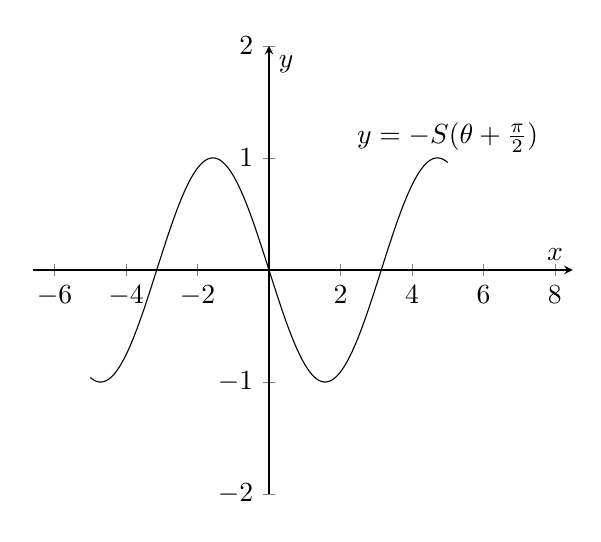
\begin{tikzpicture}
\begin{axis}[
    axis lines=middle,
    xmin=-6.6,xmax=8.5,ymin=-2,ymax=2,
    xlabel={$x$},
    ylabel={$y$}
    ]
  \addplot[samples=200] {-sin(deg(x))}node[above]{$y=-S(\theta + \frac{\pi}{2})$};
\end{axis}
\end{tikzpicture}

\textbf{Definition 13}
Let T be the function defined by T($\theta$) = $\frac{S(\theta)}{C(\theta)}$ for every real number $\theta$.

\section{Problem 33}
\textit{For what values of $\theta$ will T be undefined?}
\\ Any where $\theta$ = 2$\pi$n + 90.

\section{Problem 34}
\textit{Write down a set that is the domain of T}
\\ X $\neq$ 2$\pi$n + 90.

\section{Problem 35}
\textit{Graph T}
\\
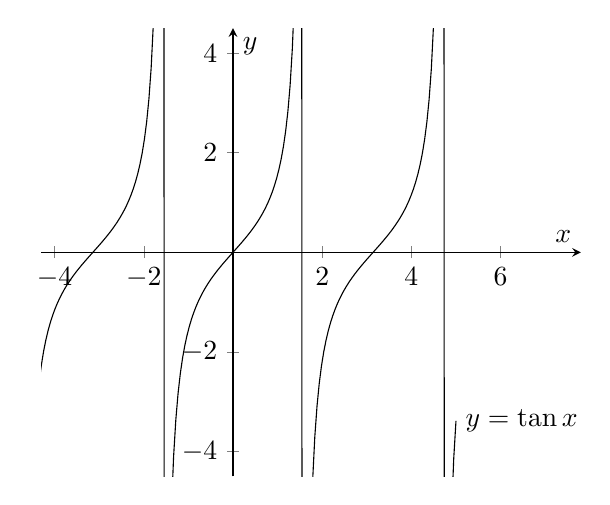
\begin{tikzpicture}
\begin{axis}[
    axis lines=middle,
    xmin=-4.3,xmax=7.8,ymin=-4.5,ymax=4.5,
    xlabel={$x$},
    ylabel={$y$}
    ]
  \addplot[samples=200] {tan(deg(x))}node[right]{$y=\tan x$};
\end{axis}

\end{tikzpicture}

\section{Problem 36}
\textit{We can skip this problem}

\section{Problem 37}
\textit{Let $\theta$ be a number such that $\theta$ is between 0 and $\frac{\pi}{2}$. Draw the unit circle, the line that is tangent to the unit circle at (1, 0), and the line that forms an angle of radian measure $\theta$ with the positive x-axis}
\\
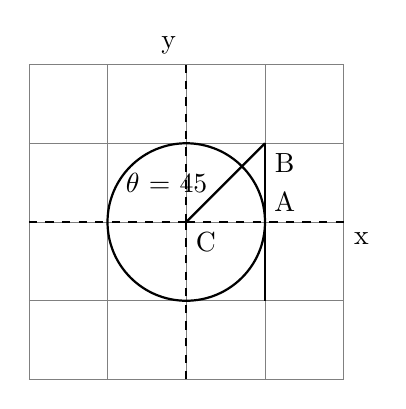
\begin{tikzpicture}
\unitcirclenolines
\draw[thick] (0,0) -- (1,1);
\draw (-.25, .5) node {$\theta$ = 45};
\draw[thick] (1,-1) -- (1, 1);
\draw (1.25, .25) node {A};
\draw (1.25, .75) node {B};
\draw (.25, -.25) node {C};
\end{tikzpicture}

\section{Problem 38}
\textit{Refer to the picture from the previous problem. Determine the length of the line segment between (1,0) and the intersection of the two lines.}
\\ \tab I can apply the tan() function. I know that $\frac{\overline{BA}}{\overline{CA}}$ must equal tan($\theta$). Since I know that tan($\theta$) = tan(45), I know that tan($\theta$) must equal 1. I already know that $\overline{CA}$ is 1. Therefore, $\overline{AB}$ must also be 1. 
\\
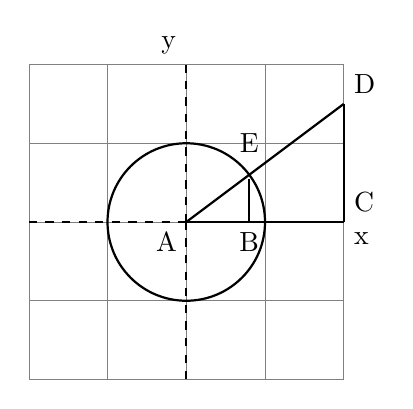
\begin{tikzpicture}
\draw[step=1cm,gray,very thin] (-2,-2) grid (2,2); %grid body
\draw[thick, dashed] (-2,0) -- (0,0); %grid line
\draw[thick, dashed] (0,-2) -- (0,0); %grid line
\draw[thick, dashed] (0,0) -- (2,0) node[anchor=north west] {x}; %axis
\draw[thick, dashed] (0,0) -- (0,2) node[anchor=south east] {y}; %axis
\draw[thick] (0,0) -- (2,1.5) node[anchor=south west] {D};
\draw[thick] (0,0) -- (2,0) node[anchor=south west] {C};
\draw[thick] (.8,.55) -- (.8, 0);
\draw(.8, -.25) node {B};
\draw(.8, 1) node {E};
\draw[thick] (2,0) -- (2,1.5);
\draw (-.25,-.25) node {A};
\draw [thick] (0,0) circle (1cm);
\end{tikzpicture}
\\ \textbf{Note: Refer to the figure above for the next three problems. Assume that the circle is a unit circle, $\theta$ is the radian measure of the angle EAB, and $\theta$ is between 0 and $\frac{\pi}{2}$.}

\section{Problem 39}
\textit{Show that S($\theta$) = l($\frac{CD}{AD}$)}.
\\ \tab
I know that triange EAB is the congruent to triangle DAC. Threrefore, $\frac{CD}{AD}$ = $\frac{BE}{AE}$. I also know that AE=1. When I look at the smaller triangle, BE is equal to S($\theta$), so this makes sense. When I scale up the lengths of AE, BE, and AB (to AD, DC and AC), I find that the theorem still holds.

\section{Problem 40}
\textit{Show that C($\theta$) = l($\frac{AC}{AD}$)}.
\\ \tab
I know that triange EAB is congruent to triangle DAC. Threrefore, $\frac{AC}{AD}$ = $\frac{AB}{AE}$. I also know that AE=1. When I look at the smaller triangle, AB is equal to C($\theta$), so this makes sense. When I scale up the lengths of AE, BE, and AB (to AD, DC and AC), I find that the theorem still holds. 

\section{Problem 41}
\textit{Show that T($\theta$) = l($\frac{CD}{AC}$)}.
\\ \tab
I know that triange EAB is congruent to triangle DAC. \\Threrefore, $\frac{CD}{AC}$ = $\frac{BE}{AB}$. Based on this knowledge, along with what we already know about sin(), cos(), and tan(), we find that T($\theta$) = l($\frac{CD}{AC}$).

We have now defined three functions, referred to as S, C, and T. 
We have also shown that if we have a right triangle with one angle of radian measure $\theta$,
 and we assume that the side adjacent to this angle has length a, the side opposite from this angle has length o, 
 and the remaining side (the hypotenuse) has length h, then these functions satisfy S( $\theta$ ) = $\frac{o}{h}$, C( $\theta$ ) = $\frac{a}{h}$, and T( $\theta$ ) = $\frac{o}{a}$. 
 
Of course, these are the three trigonometric functions sine, cosine, and tangent, that are commonly abbreviated as sin, cos, and tan, respectively. Notice that we also showed that the tangent function gets its name from the fact that it represents the length of a line segment associated with a certain line tangent to the unit circle. We now define three more functions in terms of the sine, cosine, and tangent functions.

\textbf{Definition 14.} For any number $\theta$ for which cosine is non-zero, let secant be the function defined by sec($\theta$) = $\frac{1}{cos(\theta)}$.
\textbf{Definition 15.} For any number $\theta$ for which sine is non-zero, let cosecant be the function defined by csc($\theta$) = $\frac{1}{sin(\theta)}$.
\textbf{Definition 16.} For any number $\theta$ for which cosine is non-zero, let cotangent be the function defined by cot( $\theta$ ) = $\frac{cos(\theta)}{sin(\theta)}$
\section{Problem 42}
\textit{Graph the secant function, and list the domain and range.}
\\
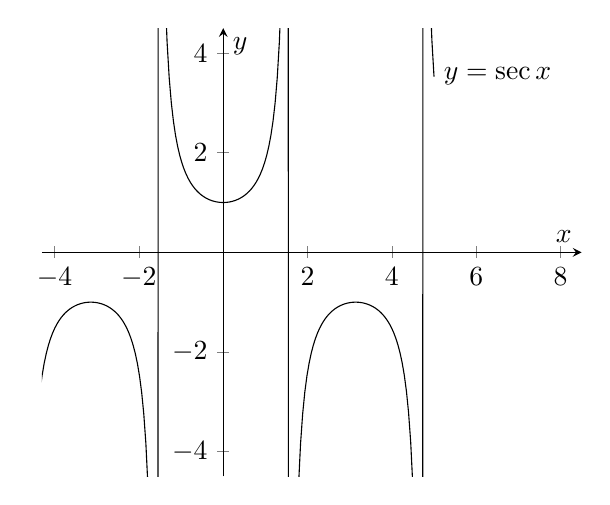
\begin{tikzpicture} \begin{axis}[
    axis lines=middle,
    xmin=-4.3,xmax=8.5,ymin=-4.5,ymax=4.5,
    xlabel={$x$},
    ylabel={$y$}
    ]
  \addplot[samples=200] {sec(deg(x))}node[right]{$y=\sec x$};
\end{axis} \end{tikzpicture}

\section{Problem 43}
\textit{Find all numbers u that satisfy 2sin(u) = 1.}
\\
This equation asks us to find all numbers for which sin(u) = $\frac{1}{2}$. We already know that this number is $\frac{\pi}{4}$+2n$\pi$ where n $\in \mathcal{Z}$.

\textbf{Note:} The previous problem could be written “Solve 2sin(u) = 1 for u”.
\section{Problem 44}
\textit{ Graph the function defined by t(x) = 3sin(x-$\pi$}
\\ \begin{tikzpicture} \begin{axis}[
    axis lines=middle,
    xmin=-4.3,xmax=10,ymin=-4.5,ymax=4.5,
    xlabel={$x$},
    ylabel={$y$}
    ]
  \addplot[samples=200] {3*sin(deg(x-3.14))}node[right]{$y=3*\sin x-3.14$};
\end{axis} \end{tikzpicture}\\
This graph makes sense because it is just like sin(x), but it is scaled up because we multiply the output of sin(x) by 3. We also shifted sin(x) to the right, by subtracting $\pi$ from x. 

\section{Problem 45}
\textit{Graph the function defined by f(x) = 5-cos(2x).}
\\ 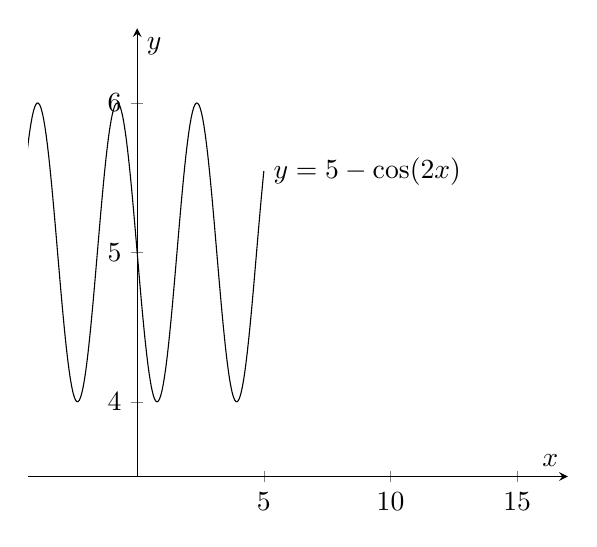
\begin{tikzpicture} \begin{axis}[
    axis lines=middle,
    xmin=-4.3,xmax=17,ymin=3.5,ymax=6.5,
    xlabel={$x$},
    ylabel={$y$}
    ]
  \addplot[samples=200] {5-sin(deg(2*x))}node[right]{$y=5-\cos(2x)$};
\end{axis} \end{tikzpicture}\\

\section{Problem 46}
\textit{Graph the function defined by r(x) = sin(x)+cos(x).}
\\ \begin{tikzpicture} \begin{axis}[
    axis lines=middle,
    xmin=-4.3,xmax=12,ymin=-2.5,ymax=2.5,
    xlabel={$x$},
    ylabel={$y$}
    ]
  \addplot[samples=200] {sin(deg(x))+cos(deg(x))}node[right]{$y=\sin x + \cos x$};
\end{axis} \end{tikzpicture}\\

\section{Problem 47}
\textit{Graph the function defined by z(u) = u*sin(u).}
\\ \begin{tikzpicture} \begin{axis}[
    axis lines=middle,
    xmin=-4.3,xmax=6,ymin=-2.5,ymax=2.5,
    xlabel={$x$},
    ylabel={$y$}
    ]
  \addplot[samples=200] {x*sin(deg(x))}node[right]{$y=u*\sin u$};
\end{axis} \end{tikzpicture}\\

\section{Problem 48}
\textit{At what minimum height above ground level must I place a satellite dish so that at a 30-degree angle, it will be able to ``see'' the sky over the top of a building that is 40 feet tall and 50 feet away from the dish?}
\\ \tab To solve this problem, I found the value of
            \begin{equation} 40 - (50tan(30)).  \end{equation}
The value of 50tan(30) tells me how high up the dish could see if it were on that ground. That value is 28.86 feet. Based on that, I can do 40  - 28.86 to find that if I mount the dish 11.132 feet off the ground, it's beam would make contact with the very top of the building. As such, it makes sense to mount the dish \textbf{A little more than 11.132 feet} off the ground.


\section{Problem 49}
\textit{Solve 2*cos($\theta$) = -$\sqrt{3}$ for $\theta$.}
\\ \tab This problem is really just asking for when cos($\theta$) = -$\frac{\sqrt{3}}{2}$. We already know that those values are:
\begin{equation}  2n\pi \pm \frac{5\pi}{6} \end{equation}
where n $\in \mathcal{Z}$. 

\section{Problem 50}
\textit{Solve tan( $\theta$ ) = 1 for $\theta$.}
\\ tan( $\theta$ ) = 1
\\ $\frac{sin(\theta)}{cos(\theta)}$ = 1
\\ sin($\theta$) = cos($\theta$)
\\ $\theta = \frac{\pi}{4}+\pi k$ where $k \in \mathcal{Z}$
\\
\\
\tab \textbf{Notation: sin\textsuperscript{n}( $\theta$ ) means (sin( $\theta$ ))n for all values of n except n = -1. In the case of n =-1, this expression represents the inverse sine function to be defined later. The same rule applies for all six of the trigonometric functions.}

\section{Problem 51} 
\textit{Solve cos\textsuperscript{2}( $\theta$ )-1 = 0 for $\theta$.}
\\
\\ cos\textsuperscript{2}( $\theta$ ) = 1
\\ cos( $\theta$ )\textsuperscript{2} = 1
\\ $\sqrt{cos(\theta)}$ = $\sqrt{1}$
\\ cos( $\theta$ ) = $\pm 1$
\\ $\theta$ = $\pi n$ where $n \in \mathcal{Z}$


\section{Problem 52}
Graph the cosecant function. 
\\ 
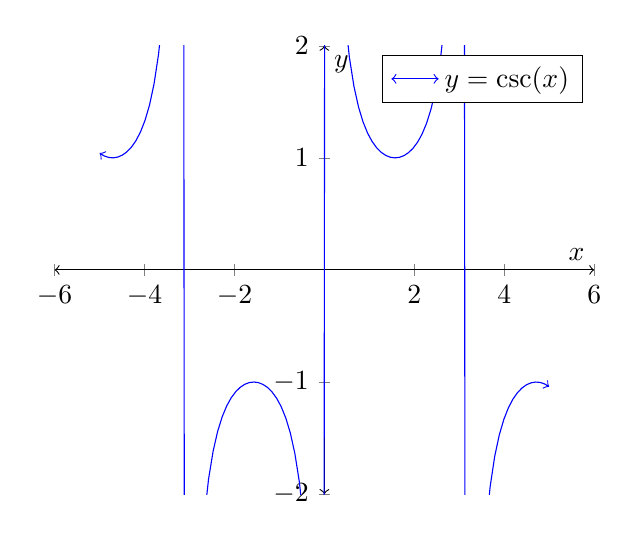
\begin{tikzpicture}
     \begin{axis}[
       xmin=-6,
       xmax=6,
       xlabel={$x$},
       ymin=-2,
       ymax=2,
       ylabel={$y$},
       axis x line=middle,
       axis y line=middle,
       axis line style=<->
     ]
       \addplot[no marks,blue,<->] expression[samples=100]{cosec(deg(x))};
       \addlegendentry{$y=\csc(x)$}; 
     \end{axis}
   \end{tikzpicture}

\section{Problem 53}
\textit{Solve sin\textsuperscript{2}(x)-sin(x) = 0 for x.}
\\
\\ sin\textsuperscript{2}(x)-sin(x) = 0
\\ sin(x)\textsuperscript{2}-sin(x) = 0
\\ sin(x)\textsuperscript{2}-sin(x) = 0
\\ sin(x)\textsuperscript{2} = sin(x)
\\ sin(x) must equal 0 or 1. sin(x) $\neq$ -1, as -1*-1 $\neq$ -1.
\\ sin(x) = $\pi n$ or $2\pi n + \frac{\pi}{2}$, where n $\in \mathcal{Z}$


\section{Problem 54} 
\textit{Solve 2sin\textsuperscript{2}$(\frac{x}{2}$)-3sin\textsuperscript{2}($\frac{x}{2}$)+1 =0 for x.}
\\
\\2sin\textsuperscript{2}$(\frac{x}{2}$)-3sin\textsuperscript{2}($\frac{x}{2}$)+1 =0
\\2sin$(\frac{x}{2})$\textsuperscript{2}-3sin($\frac{x}{2}$)\textsuperscript{2}+1 =0
\\Here, sin$(\frac{x}{2})$\textsuperscript{2} must equal 1. So, I can solve for 
\\ sin$(\frac{x}{2})$\textsuperscript{2} = 1
\\ $\sqrt{sin(\frac{x}{2})\textsuperscript{2}}$ = $\pm$1
\\ sin$(\frac{x}{2})$ = $\pm$1
\\ So, x = 2n$\pi$, where n $\in \mathcal{Z}$


\section{Problem 55}
\textit{Krista is standing at the edge of a long straight beach when she sees Jared drowning. Assume that Jared is at a distance of 76 meters straight out from a point on the beach that is 380 meters from where Krista is standing. Assume that Krista can run at 6.5 meters per second and swim at 1.4 meters per second. Krista runs down the beach toward Jared to a point P on the beach, and then dives into the water and swims to Jared. The angle at the point P between the beach and the line from P to Jared has a measure of 77 degrees. How long does it take Krista to save Jared? Could she have saved him faster by taking a different path?}
\\ ??


\section{Problem 56} \textit{Graph cotangent, and list its domain and range.}
\\
\begin{tikzpicture}
     \begin{axis}[
       xmin=-6,
       xmax=6,
       xlabel={$x$},
       ymin=-2,
       ymax=2,
       ylabel={$y$},
       axis x line=middle,
       axis y line=middle,
       axis line style=<->
     ]
        \addplot[no marks,blue,<->]expression[samples=100]{$1/\tan(deg(x))$};
       \addlegendentry{$y=cotan(x)$};
	\end{axis}
\end{tikzpicture}
\\
Domain: $\mathds{R}$
\\ Range: Y $>$ 1 or Y $<$ -1. 

\section{Problem 57} \textit{Solve cot($\theta$) $>$ 0 for $\theta$}
\\
$\pi n<x<\pi n + \frac{\pi}{2}, n \in \mathcal{Z}$
\\
If $\theta = \pi$, then sin($\theta$)=0, and the equation would be undefined. If $\theta = \frac{\pi}{2}$, then cos($\theta$) would be 0, and $\frac{0}{sin(\theta)}$ would equal 0. 
\begin{comment}
\section{Problem 58}
\textit{Graph the function defined by f(x) = 3-2sin(2x+$\pi$ ).}
\begin{tikzpicture}
     \begin{axis}[
       xmin=-6,
       xmax=6,
       xlabel={$x$},
       ymin=-2,
       ymax=2,
       ylabel={$y$},
       axis x line=middle,
       axis y line=middle,
       axis line style=<->
     ]
       \addplot[no marks,blue,<->] expression[samples=100]{$y = 3-2\sin(2*deg(x)+3.14)$};
       \addlegendentry{y=f(x)};
	\end{axis}
\end{tikzpicture}

\end{comment}

\newpage
\section*{For Reference:}

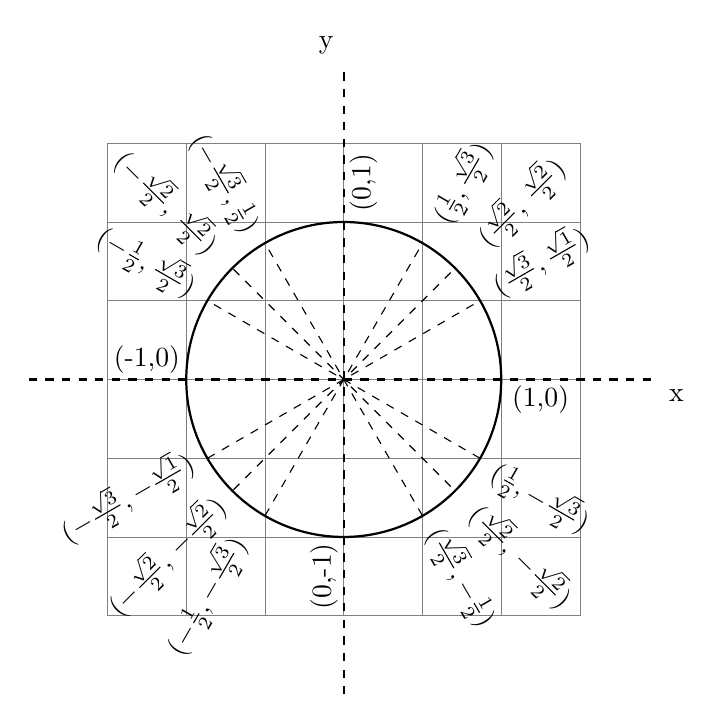
\begin{tikzpicture}
\unitcircle
\end{tikzpicture}

\end{document}

